\documentclass{article}
\usepackage {mathtext}
\usepackage{amsmath}
\usepackage [russian] {babel}
\usepackage{caption}
\captionsetup[table]{position=t,justification=raggedleft,slc=off}
\setlength{\abovecaptionskip}{0pt}
\usepackage {geometry}
\usepackage {amssymb}
\usepackage{graphicx}
\geometry{left=3cm, right=1.5cm, top=2cm, bottom=2cm}
\title{Лабораторная работа №3.4.2. \\ \textbf{Закон Кюри-Вейсса}}
\author{Михаил Орлов, Павел Рудачихин, Б04-507}
\date{01.09.2026}
\begin {document}
\maketitle{}


\section {Аннотация} 
	\hspace{4mm} Целью данной работы являются проверка температурной зависимости магнитной восприимчивости гадолиния около точки Кюри (закон Кюри-Вейсса) и определение парамагнитной и ферромагнитной точек Кюри для гадолиния. Метод основан на том, что образец гадолиния, будучи сердечником катушки LC-автогенератора, меняет свою магнитную восприимчивость  при изменении температуры. Следовательно, изменяется индуктивность катушки и период автоколебаний.

\section {Теоретическое введение}

	\hspace{4mm} Для парамагнетиков с хорошей точностью выполняется закон
	
	\begin{equation}
		\vec{M} = \chi \vec{H},
	\end{equation}
	
	где $\vec{M}$ -- вектор \textit{намагниченности}, равный магнитному моменту единичного объёма вещества, $\vec{H}$ -- \textit{напряжённость} поля, $\chi > 0$ -- \textit{магнитная восприимчивость}. 
	
	
	Из выражения для энергии магнитного диполя с модулем магнитного момента $m$ и углом $\alpha$ к магнитному полю с индукцией $B$: $U(\alpha) = -mB\cos\alpha$, и распределения Больцмана имеем \textit{закон Кюри}
	
	\begin{equation}
		\chi \propto \frac{1}{T}
	\end{equation}
	
	
	Помимо парамагнетиков существуют \textit{ферромагнетики} -- вещества, сильно намагничивающиеся даже в небольших магнитных полях и имеющие нелинейную зависимость $M(H)$. Происходит это потому, что в отсутствие внешнего магнитного поля атомы ферромагнетика способны образовывать упорядоченные структуры с практически однонаправленной ориентацией всех магнитных моментов -- \textit{домены}. 
	
	
	Поведение ферромагнетиков можно описать с помощью \textit{модели среднего поля}. Согласно ей, намагниченность элемента среды пропорциональна эффективному полю $\vec{H_e}$, складывающемуся из внешнего поля $\vec{H}$ и среднего поля <<соседей>>, пропорционального намагниченности $\vec{M}$ с коэффициентом $\beta$. Тогда можно считать отдельный атом в эффективном поле парамагнетиком с магнитной восприимчивостью $\chi_p$:
	
	\begin{equation}
		\vec{M} = \chi_p \vec{H_e} = \chi_p(\vec{H} + \beta\vec{M})
	\end{equation}
	
	
	Определив магнитную восприимчивость аналогично (1), получаем закон Кюри-Вейсса:
	
	\begin{equation}
		\chi \propto \frac{1}{T - \Theta},
	\end{equation}
	
	где $\Theta$ имеет размерность температуры.
	
	Закон Кюри-Вейсса предсказывает существование температуры $\Theta_K$, называемой \textit{точкой Кюри}, в которой $\chi \rightarrow \infty$, т.е. происходит фазовый переход второго рода между парамагнитным и ферромагнитным состояниями вещества. Но модель среднего поля в этих условиях становится слишком грубой, поэтому $\Theta \neq \Theta_K$ и имеет место зависимость, изображённая на рисунке 1. $\Theta = \Theta_p$ называется \textit{парамагнитной точкой Кюри}.
	
	\begin{figure}[h!]
		\centering
		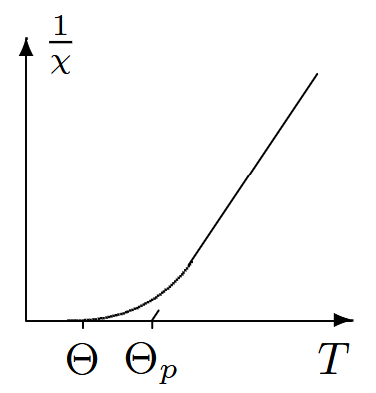
\includegraphics[width=0.3\linewidth]{1}
		\caption{Зависимость обратной величины магнитной восприимчивости от температуры}
		\label{fig:1}
	\end{figure}
	
	
	В работе изучается температурная зависимость $\chi(T)$ гадолиния, чья точка Кюри лежит в диапазоне комнатных температур. 
	
	
\section{Описание установки}

	\hspace{4mm} В настоящей работе используются катушка с образцом гадолиния, термостат, частотомер, вольтметр, LC-автогенератор и медно-константановая термопара.
	
	\begin{figure}[h!]
		\centering
		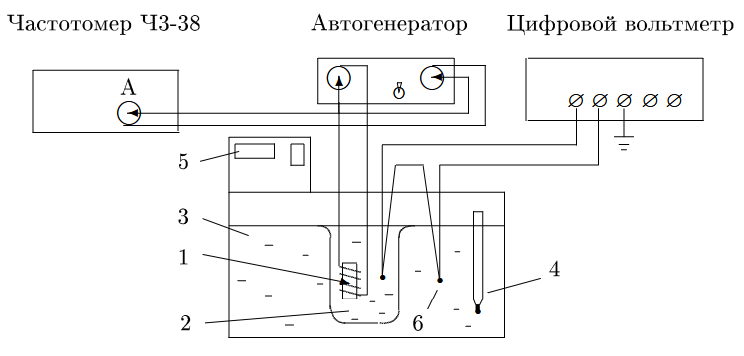
\includegraphics[width=0.7\linewidth]{2}
		\caption{Схема установки: 1 - катушка с образцом, 2 - сосуд с трансформаторным маслом, 3 - рабочая жидкость термостата, 4 - ртутный термометр, 5 - термостат.}
		\label{fig:2}
	\end{figure}
	
	
	 Схема установки приведена на рисунке 2. Образец гадолиния расположен внутри пустотелой катушки 1, которая служит индуктивностью LC-автогенератора. Катушка помещена в стеклянный сосуд 2 с трансформаторным маслом. Масло предохраняет образец от окисления, ухудшает электрический контакт между его частичками и улучшает тепловой контакт с рабочей жидкостью 3 термостата 5.
	
	
	Коэффициент самоиндукции катушки $L$ пропорционален магнитной проницаемости $\mu$ заполняющей её среды, откуда
	
	\begin{equation}
		L - L_0 \propto \mu - 1 = \chi,
	\end{equation}
	 
	 где $L_0$ - самоиндукция катушки без образца.
	 
	 
	 При изменении индуктивности меняется период автогенератора $\tau$. Отсюда
	 
	 \begin{equation}
	 	\frac{1}{\tau^2 - \tau_0^2} \propto T - \Theta_p
	 \end{equation}
	 
	Температура образца отличается от температуры рабочей жидкости термостата. Для контроля этой разности используется медьно-константановая пара 6 и вольтметр.
	 
	 
	Для используемой в работе установки чувствительность термопары $\kappa =24\ К/мВ$, период колебаний LC-автогенератора без образца $\tau_0 = (9,045 \pm 0,005) \ мкс$
	
\section{Результаты и обсуждения}

	\hspace{4mm} В ходе выполнения лабораторной работы была снята зависимость $\tau(t)$ в 9 точках в диапазоне 14 -- 34 $^oС$ (см. Приложение). Он меньше рекомендуемого 14 -- 40 $^oС$. Сужение было обусловлено дефицитом времени на выполнение работы, но позже было установлено, что в оставшемся отрезке 34 -- 40  $^oС$ погрешность величины $(\tau^2 - \tau_0^2) ^{-1}$ оказалась бы слишком высокой (уже при $t = 34\ ^oС $ относительная погрешность составила 8\%). Поэтому принятое решение не повлияло на результат -- 5 точек на линейном участке оказалось достаточно.
	
	\begin{figure}[h!]
		\centering
		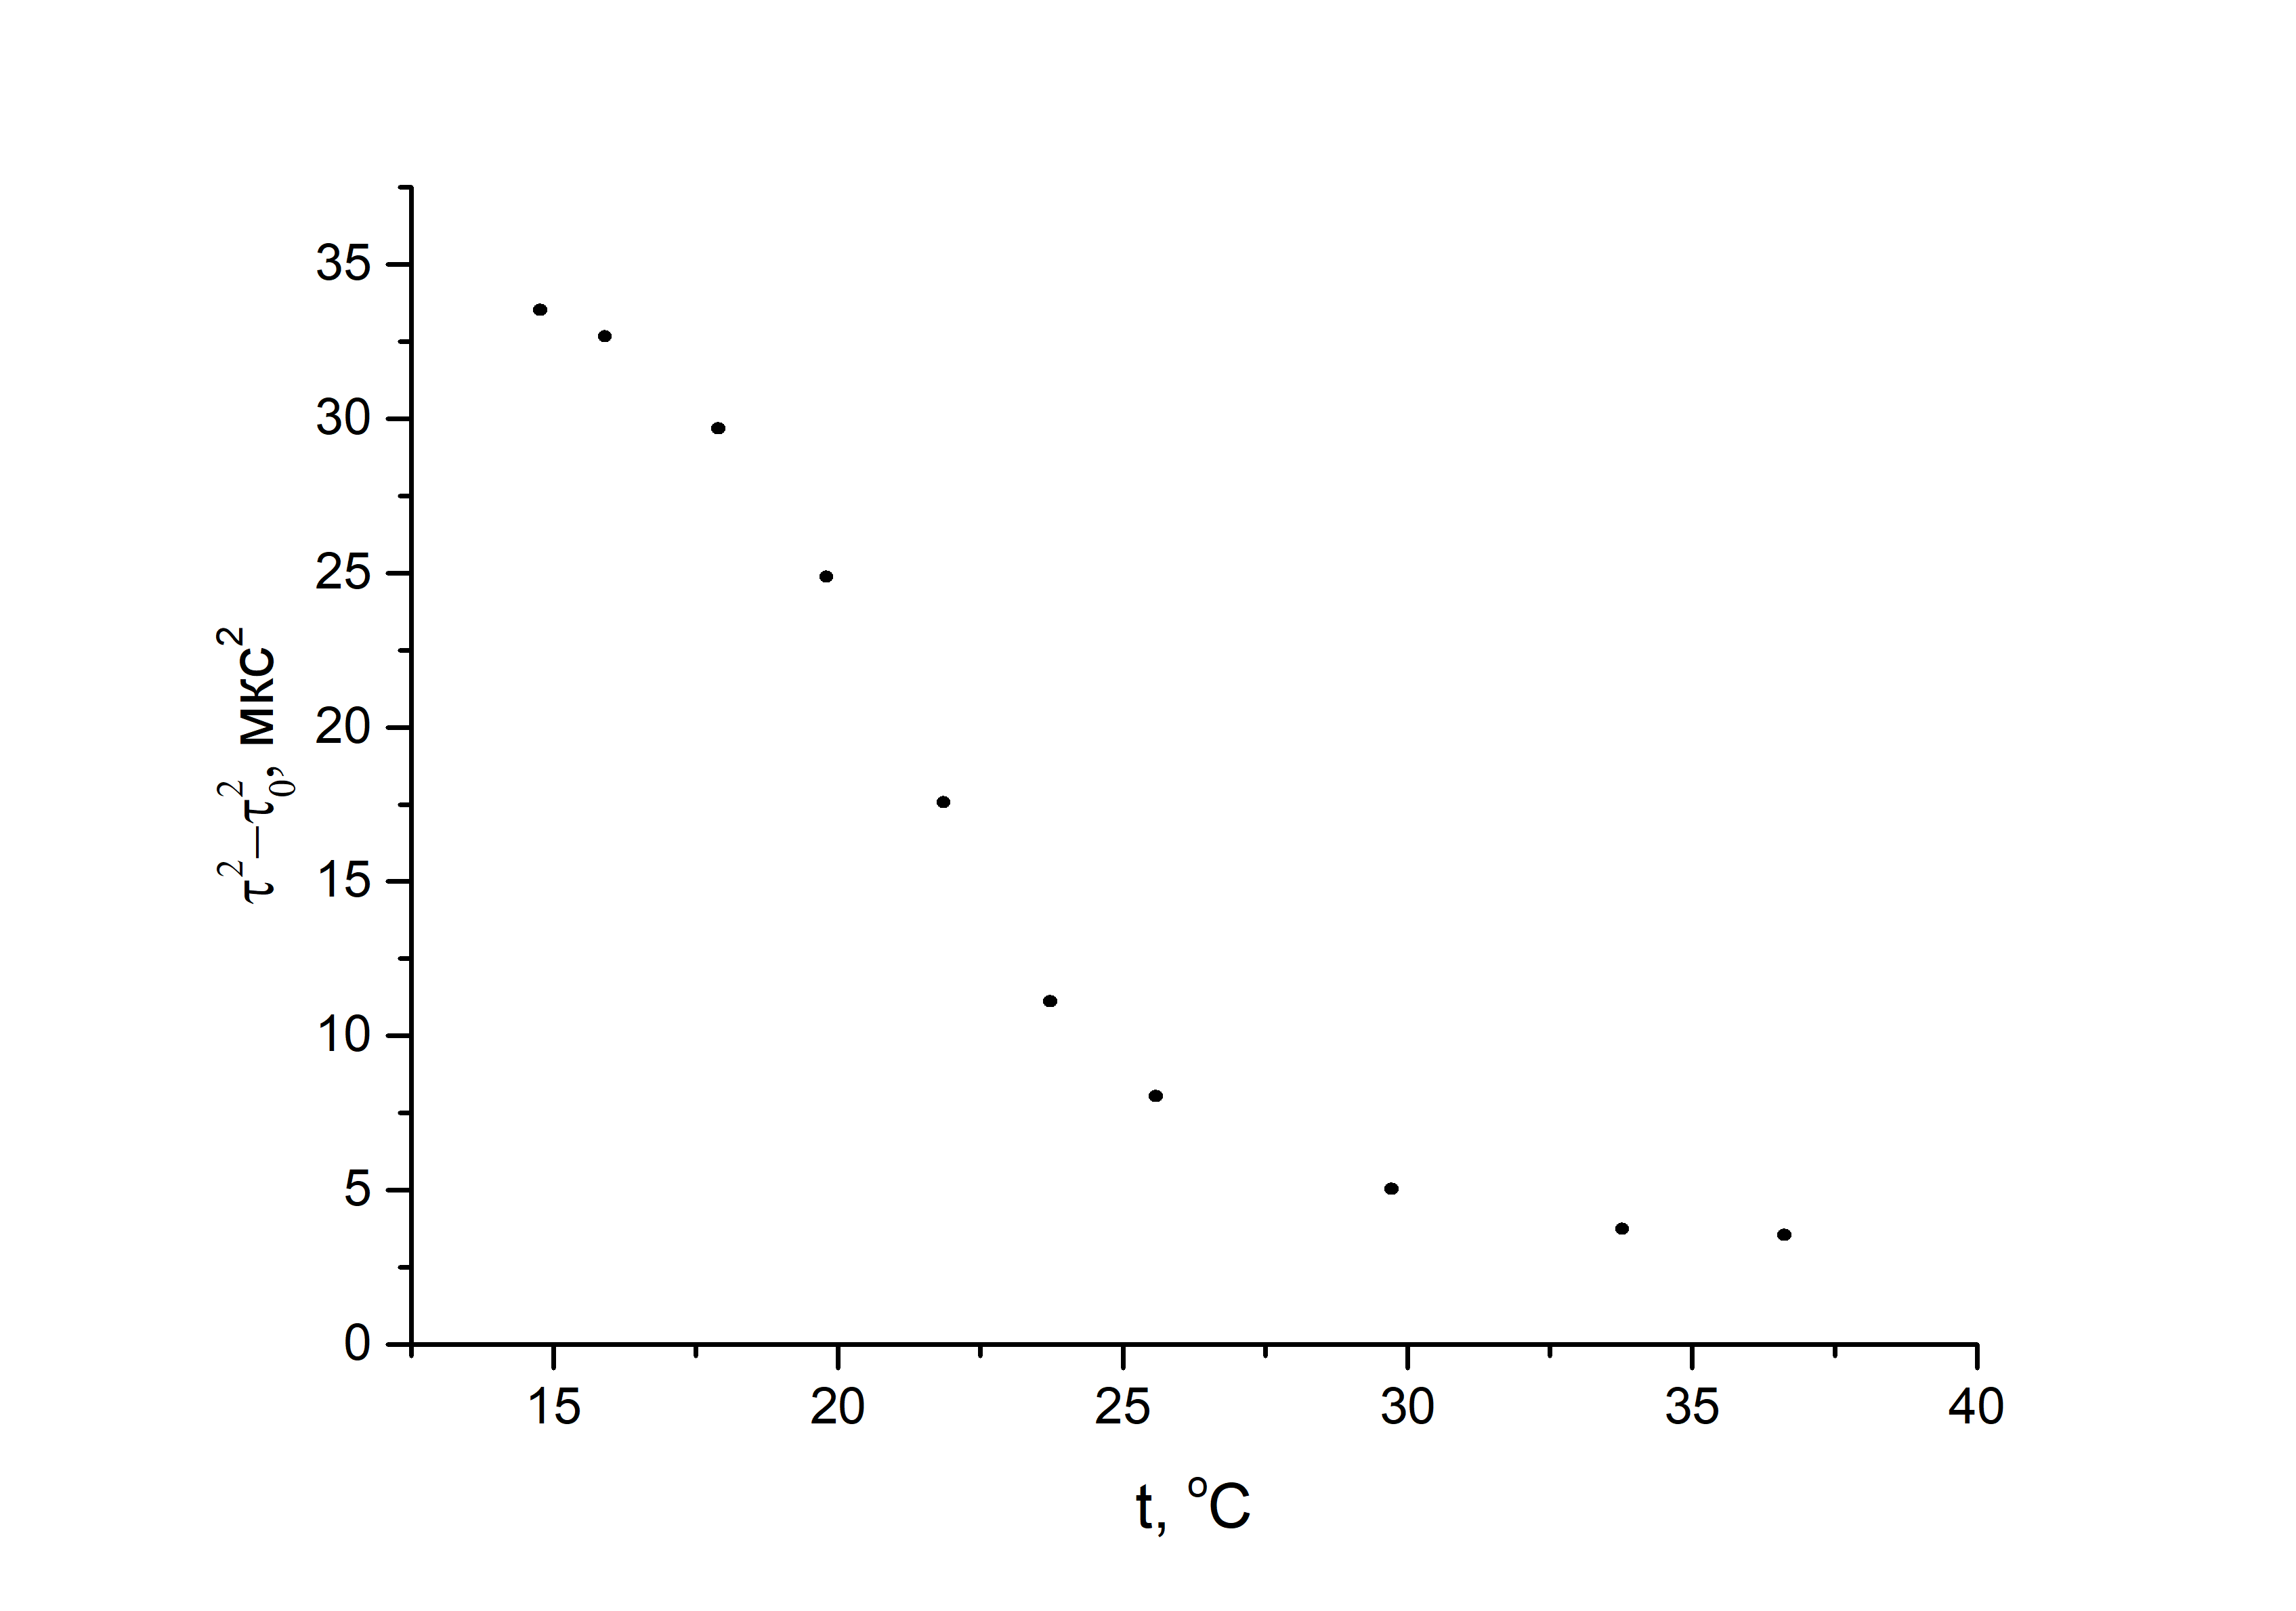
\includegraphics[width=0.8\linewidth]{4}
		\caption{Зависимость $\tau^2 - \tau_0^2 =  f(t)$}
		\label{fig:4}
	\end{figure}
	
	Для каждой точки была зафиксирована $\Delta U$ -- ЭДС термопары. Измерения производились после установления допустимой $|\Delta U| < 0,5 \ К \ / \ (24 \ К/мВ) = 0,021 \ мВ$.
	
	
	Частотомер отображал значение периода в мкс с точностью 5 знаков после запятой, но из-за быстрых изменений значений в последних 3 разрядах погрешность положена равной $\sigma(\tau) = 0,005$ мкс. Эти изменения могут быть связаны как со случайной погрешностью измерения (например, проводник, соединяющий автогенератор с контактами вольтметра, довольно длинный, что усиливает влияние помех на измерение), так и непосредственно с изменением периода вследствие уменьшения разности температур образца и термостатирующей жидкости. Поэтому, возможно, при более долгом ожидании флуктуации показаний уменьшились бы. 
	
	
	Погрешности цифрового термометра термостата и вольтметра определены по последнему разряду и положены $\sigma(t) = 0,01 \ ^oС; \ \sigma(\Delta U) = 0,001 \ мВ$.
	
	
	Из графика зависимости $\tau^2 - \tau_0^2 =  f(t)$ (рис. 3) следует, что фазовый переход второго рода из ферромагнитного состояния в парамагнитное происходит в интервале температур 16 -- 30 $^oC$. 
	
	
		\begin{figure}[h!]
		\centering
		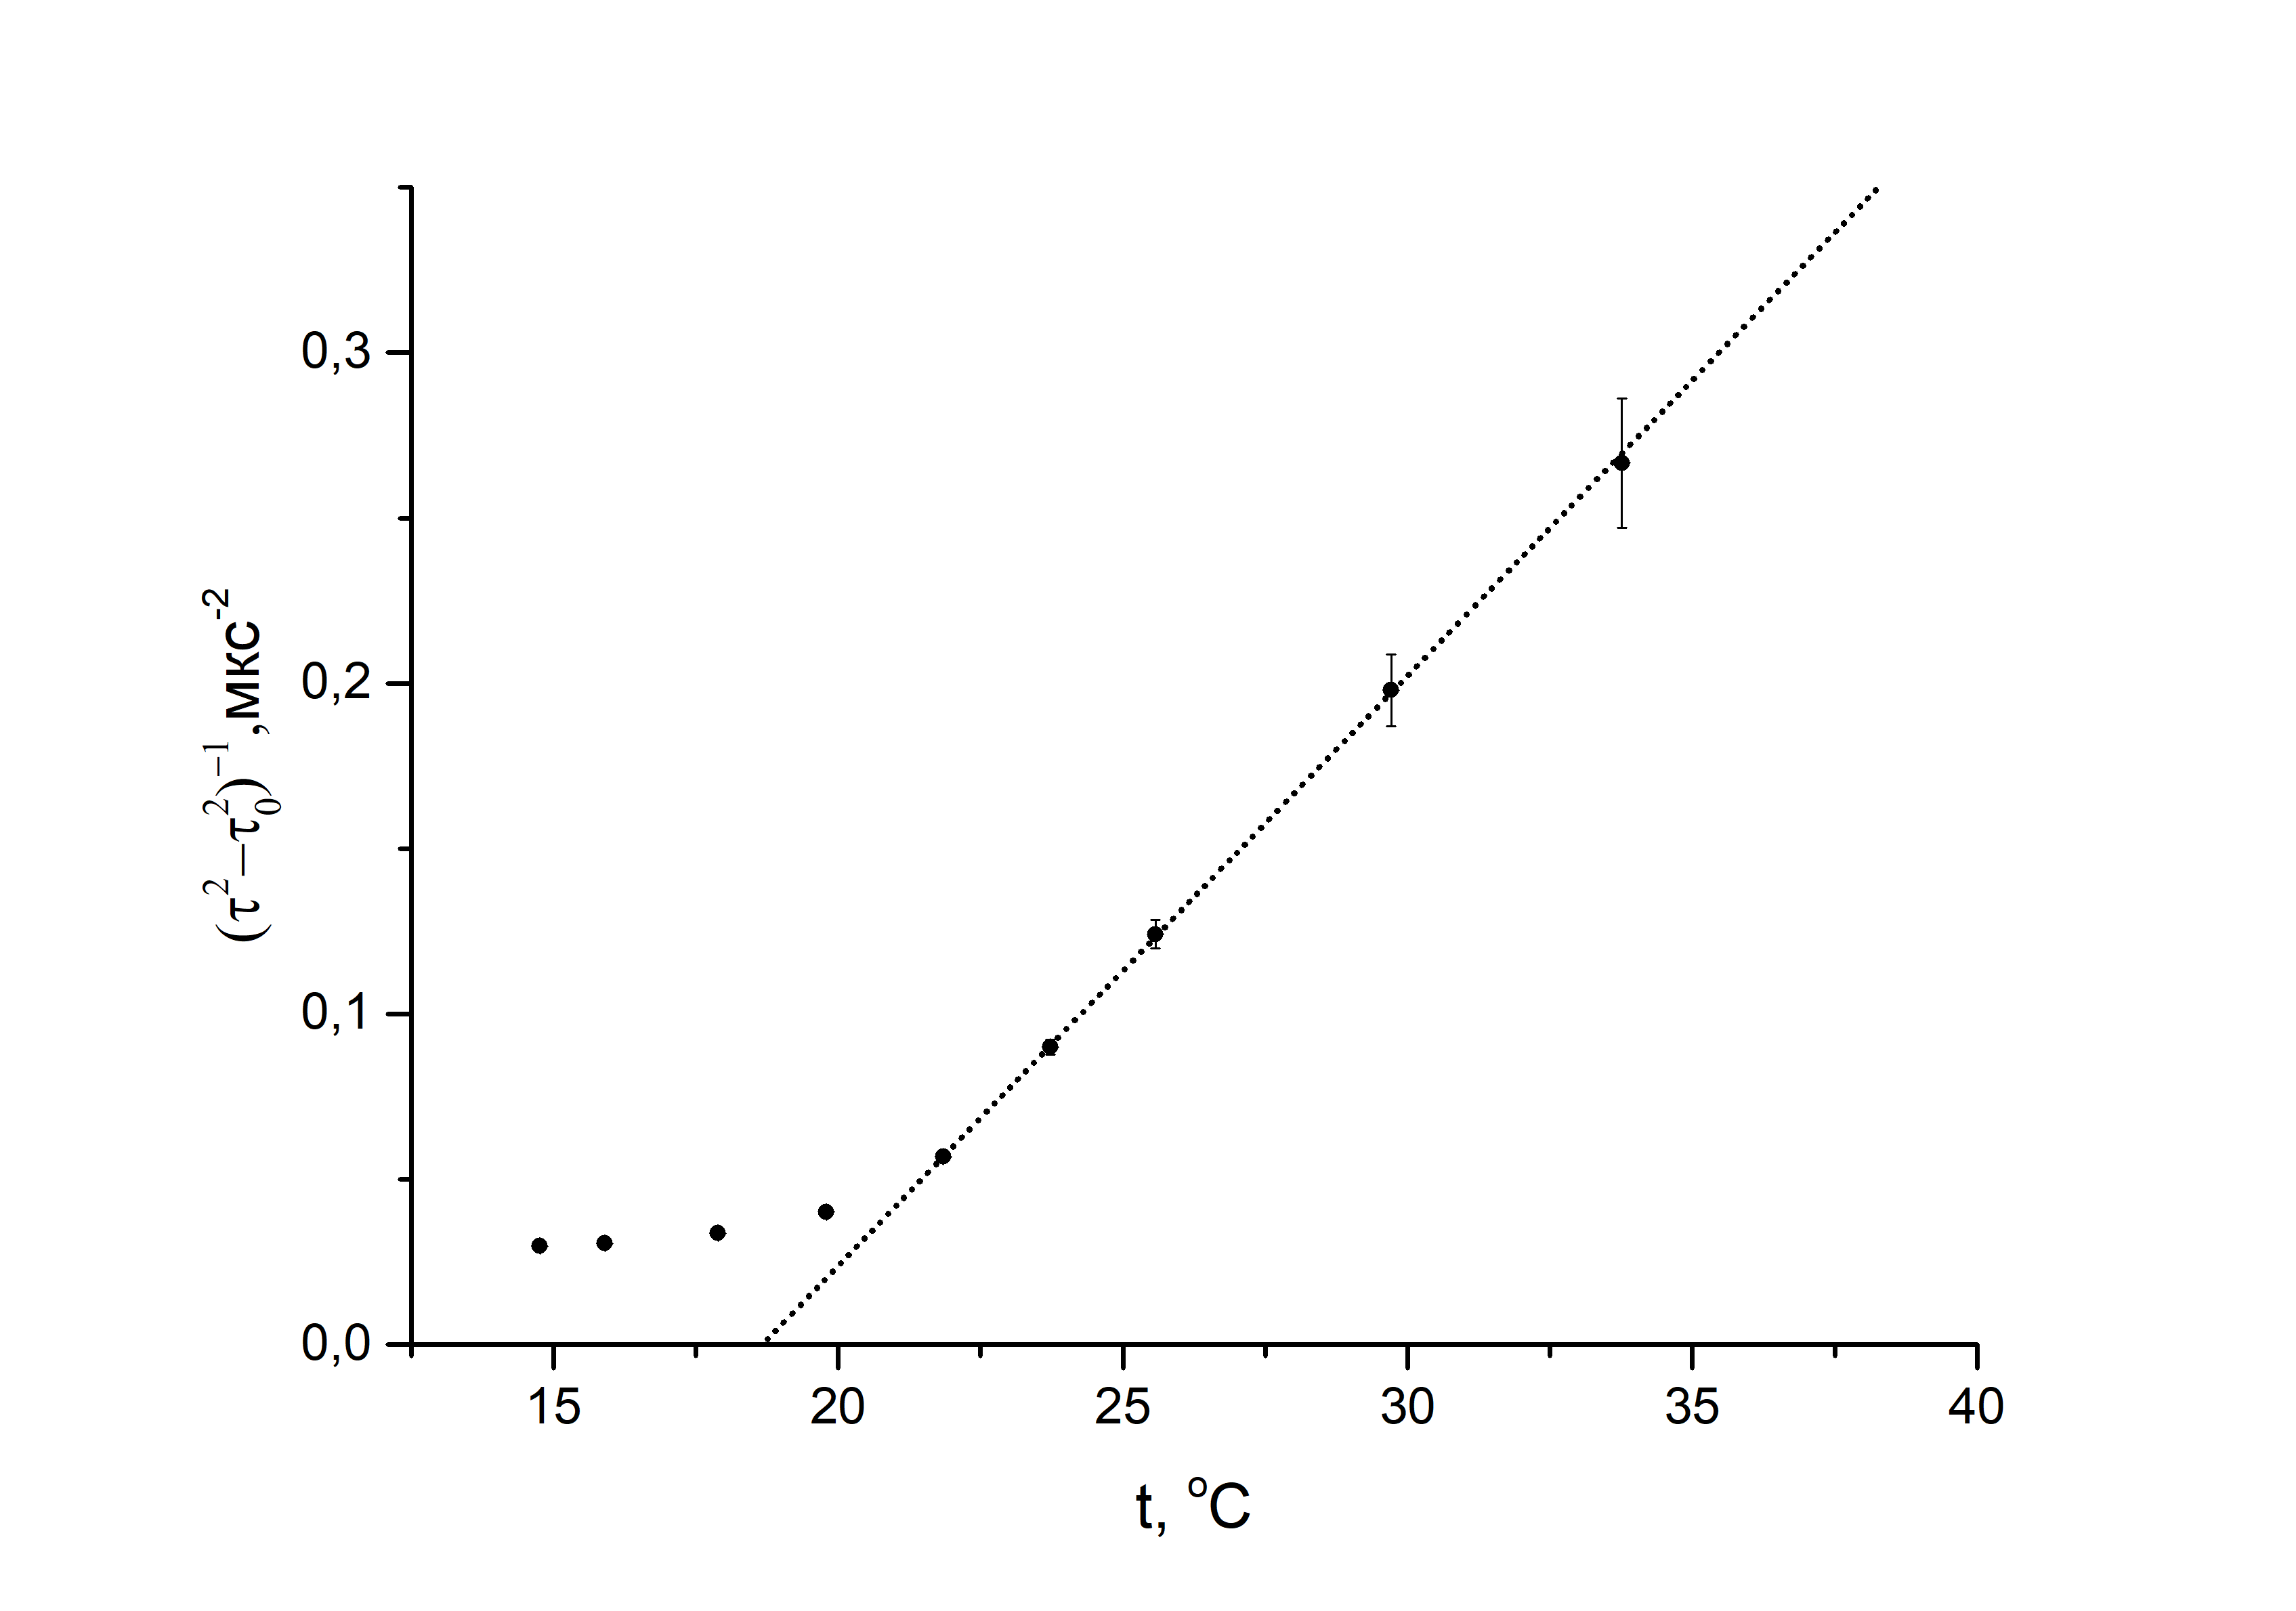
\includegraphics[width=0.8\linewidth]{3}
		\caption{Зависимость $(\tau^2 - \tau_0^2) ^{-1} =  f(t)$}
		\label{fig:3}
	\end{figure}
	
	На графике зависимости $(\tau^2 - \tau_0^2) ^{-1} =  f(t)$ (рис. 4) проведена прямая по методу наименьших квадратов через последние 5 точек. По её пересечению с осью абсцисс установлено значение параметрической точки Кюри
	
	\[\Theta_p = (18,6 \pm 0,2) \ ^oС  \] 
	
	По тому же графику можно оценить температуру точки Кюри как начало перехода к линейному возрастанию
	
	
	\[\Theta = (19,8 \pm 1,0) \ ^oС  \]
	

\section{Выводы}

	\hspace{4mm} По 9 экспериментальным точкам был построен график $(\tau^2 - \tau_0^2) ^{-1} =  f(t)$, по которому удалось проверить справедливость закона Кюри-Вейсса (4) с помощью $(\tau^2 - \tau_0^2) ^{-1} \propto \chi$.
	
	По линейному участку этого графика определена парамагнитная точка Кюри $\Theta_p = (18,6 \pm 0,2) \ ^oС  $. Она ожидаемо оказалась близка к точке Кюри $\Theta = (19,8 \pm 1,0) \ ^oС$. Точка Кюри определена двумя способами: по обнаружению фазового перехода на графике $\tau^2 - \tau_0^2 =  f(t)$ и по переходу к линейной зависимости на графике $(\tau^2 - \tau_0^2) ^{-1} =  f(t)$. Последний оказался гораздо точнее. 
	
	Полученная оценка точки Кюри $\Theta = (19,8 \pm 1,0) \ ^oС$ совпадает с табличным значением $20,2\ ^oС$ в пределах погрешности.
	
	Основным источником погрешности эксперимента стали изменения показаний частотомера. В связи с этим предложено улучшить помехоустойчивость установки и увеличить ожидание теплового равновесия образца и термостатирующей жидкости.   




\section{Приложение. Результаты измерений}




\begin{table}[h!]
	
	\centering
	\begin{tabular}{|c|c|c|}
		\hline
		$t, ^oC$ & $- \Delta U, \ мВ$ & $\tau, \ мкс$ \\
		\hline
		14,88 & 0,005 & 10,74 \\
		\hline
		16,02 & 0,005 & 10,70 \\
		\hline
		18,06 & 0,007 & 10,56 \\
		\hline
		20,03 & 0,010 & 10,33 \\
		\hline
		22,04 & 0,008 & 9,97 \\
		\hline
		24,01 & 0,012 & 9,64 \\
		\hline
		25,93 & 0,015 & 9,48 \\
		\hline
		30,02 & 0,013 & 9,32 \\
		\hline
		34,05 & 0,012 & 9,25 \\
		\hline
		36,00 & 0,012 & 9,24 \\
		\hline
	\end{tabular}
\end{table}




\end {document}